\documentclass{article}
\usepackage[utf8]{inputenc}

\title{Assignment-8\\Synchronization Problems}
\author{Subash Mylraj \\(CED18I051) }
\date{30 November 2020}

\usepackage{geometry}
 \geometry{
 a4paper,
 total={170mm,257mm},
 left=20mm,
 top=10mm,
 }

\usepackage{longtable}
\usepackage{graphicx}
\usepackage{listings}
\usepackage{xcolor}

\begin{document}

\maketitle

\lstset{
  language=c,
  aboveskip=3mm,
  belowskip=3mm,
  showstringspaces=false,
  columns=flexible,
  basicstyle={\small\ttfamily},
  numbers=none,
  numberstyle=\tiny\color{gray},
  keywordstyle=\color{blue},
  commentstyle=\color{dkgreen},
  stringstyle=\color{mauve},
  breaklines=true,
  breakatwhitespace=true,
  tabsize=3
}

\definecolor{dkgreen}{rgb}{0,0.6,0}
\definecolor{gray}{rgb}{0.5,0.5,0.5}
\definecolor{mauve}{rgb}{0.58,0,0.82}

\section*{Dining Philosopher problem}
\bigskip

\par\noindent
\textbf{\Large Code:}
\smallskip
\par\noindent\rule{\textwidth}{0.4pt}
\lstinputlisting[language=c]{src/dining_philosopher.c}
\par\noindent\rule{\textwidth}{0.4pt}

\bigskip
\noindent
\textbf{\Large Output:}

\begin{figure}[h]
	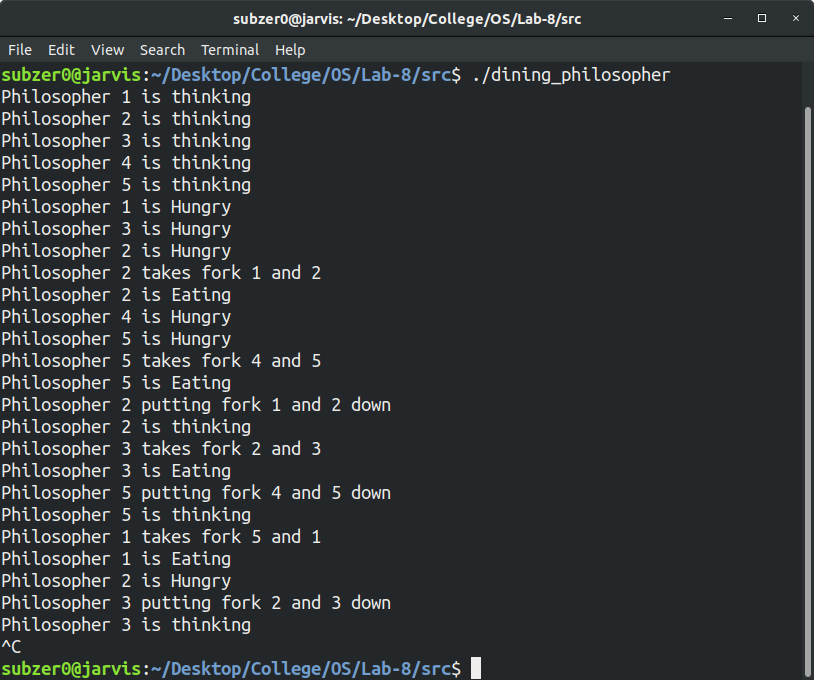
\includegraphics[width=\textwidth]{output/dining_philosopher.png}
\end{figure}
\bigskip

\section*{Reader Writer problem}

\par\noindent
\textbf{\Large Code:}
\smallskip
\par\noindent\rule{\textwidth}{0.4pt}
\lstinputlisting[language=c]{src/reader_writer.c}
\par\noindent\rule{\textwidth}{0.4pt}

\bigskip
\noindent
\textbf{\Large Output:}

\begin{figure}[h]
	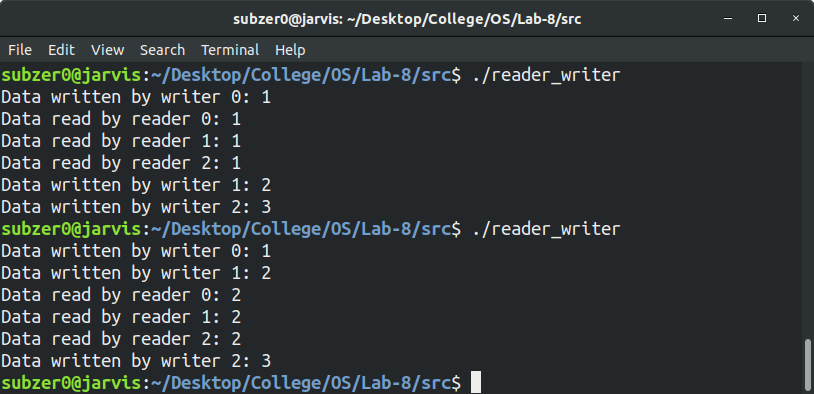
\includegraphics[width=\textwidth]{output/reader_writer.png}
\end{figure}
\bigskip
\pagebreak

\section*{H2O problem}
\par\noindent
\textbf{\Large Code:}
\smallskip
\par\noindent\rule{\textwidth}{0.4pt}
\lstinputlisting[language=c]{src/h2o.c}
\par\noindent\rule{\textwidth}{0.4pt}

\bigskip
\noindent
\textbf{\Large Explanation: } \\

The size of hydroqueue is 2 and that of oxyqueue is 1. As the first two hydrogen threads arrive, they
get pushed to the hudrogen queue, and as the first oxygen queue arrives, it gets pushed to the oxygen
queue. Once the requirement to bond is achieved (2 x hydrogen and 1 x oxygen), the threads call where 
they bond after which they are moved to the barrier to make sure that the bonded hydrogen and oxygen
are accounted for.

The forthcoming hydrogen and oxygen threads are made to wait until the their respective queues can
accmodate them.

\bigskip
\noindent
\textbf{\Large Output:}

\begin{figure}[h]
	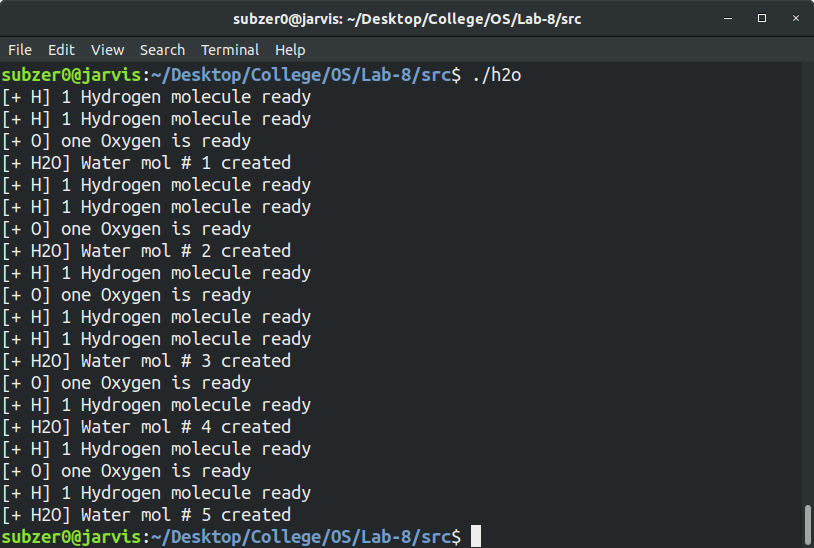
\includegraphics[width=\textwidth]{output/h2o.png}
\end{figure}
\bigskip

\section*{Senate problem}
\par\noindent
\textbf{\Large Code:}
\smallskip
\par\noindent\rule{\textwidth}{0.4pt}
\lstinputlisting[language=c]{src/senate.c}
\par\noindent\rule{\textwidth}{0.4pt}

\bigskip
\noindent
\textbf{\Large Explanation: } \\

We set the maximum number of riders by the $MAX\_RIDERS$ constant. The global variable 
waiting is incremented as riders arrive at the station. Once the bus arrives, waiting
is decreased for each rider that is at the station. A mutex lock $riders\_waiting$ is acquired
by the bus when it has arrived, hence not allowing more riders to enter the station. 
$bus\_arrival$ and $bus\_depart$ are semaphores that are used to communicate between the riders
and the bus to know whether all the riders at the station have entered or not.


\bigskip
\noindent
\textbf{\Large Output:}

\begin{figure}[h]
	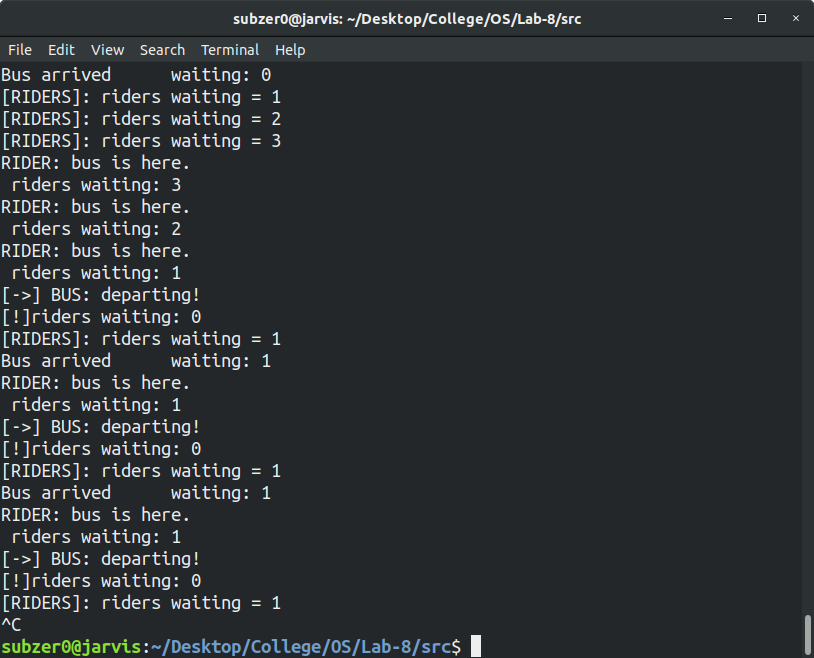
\includegraphics[width=\textwidth]{output/senate.png}
\end{figure}
\bigskip

\end{document}